\documentclass[11pt,twocolumn]{article}
\usepackage{verbatim}
\usepackage[utf8]{inputenc}
\usepackage{caption}
\usepackage[T1]{fontenc}
\usepackage{graphicx}
\usepackage[spanish,es-tabla,es-nodecimaldot]{babel}
\usepackage{csquotes}
\usepackage{amssymb}
\usepackage{amsbsy}
\usepackage[version=4]{mhchem} %notacion quimica /ce
\usepackage{hyperref}
\usepackage{placeins} %para el floatbarrier
\usepackage{url}
%\usepackage{dblfloatfix}
\usepackage{multirow}
\usepackage{amsmath}
\usepackage{tikz}
\usepackage[sc]{mathpazo}
\linespread{1.05}
\usepackage{siunitx}
\usepackage[letterpaper,top=2.5cm,bottom=2cm,left=1.3cm,right=1.5cm,marginparwidth=1.75cm]{geometry}

\setlength{\marginparwidth}{2cm}
\usepackage[colorinlistoftodos]{todonotes}
%\usepackage{epstopdf}
\usepackage{units}
%paquete para enumerar con letras
\usepackage[shortlabels]{enumitem}
\usepackage{float}
\usepackage{blindtext}
\usepackage{microtype}
\usepackage{makecell}
\usepackage{lettrine}
\usepackage{titling}
\usepackage{booktabs}
\usepackage{ragged2e}
\usepackage{cuted}
\usepackage{authblk}
\usepackage{adjustbox}
\usepackage{xcolor}
\usepackage{lipsum}
%pa que pueda numerar dentro de align*
%\newcommand\numberthis{\addtocounter{equation}{1}\tag{\theequation}}
\usepackage[normalem]{ulem}
\usepackage{lscape}
\usepackage{tabularx}
\usepackage{cancel}
\usepackage{lmodern}%get scalable font
\usepackage{dsfont}
\usepackage{lipsum}
\usepackage{relsize}
\usepackage{comment}
\usepackage{physics} % para la notacion bra y ket
\usepackage{mathtools} % para hacer la flecha en ambas direcciones
\usepackage{tablefootnote}
%\usepackage{gensymb} % para el simbolo °
\usepackage{derivative}%ecuaciones diferenciales de grado n usar \odv[n]{f}{x} y parciales de grado n \pdv[n]{f}{x}
\setlist[itemize]{noitemsep}
\usepackage{abstract}
\renewcommand{\abstractnamefont}{\normalfont\bfseries}
\renewcommand{\abstracttextfont}{\normalfont\small\itshape}
\usepackage{titlesec}% Allows customization of titles

\titleformat{\section}[hang]{\large\centering}{\thesection.}{1em}{} % Change the look of the section titles

\titleformat{\subsubsection}[block]{\large}{\thesubsubsection.}{1em}{} % Change the look of the subsubsection titles

% Allows customization of titles
\usepackage[labelfont=bf,textfont=it]{caption}
\usepackage{subcaption}

\titleformat{\subsection}[block]{\large}{\thesubsection.}{1em}{}
% Change the look of the section titles
\setlength{\droptitle}{-4\baselineskip}
% Move the title up
\usepackage{hyperref}
\usepackage{listings}
\hypersetup{
    colorlinks=true,
    citecolor=blue,
    filecolor=blue,
    urlcolor=blue,
    allcolors=blue
}

\usepackage{cleveref}
\usepackage[
	backend = biber,
	bibencoding = utf8,
	sorting = none
]{biblatex}
% \usepackage[backend=bibtex]{biblatex}
\newcommand{\angstrom}{\textup{\AA}}
\addbibresource{bibliogra.bib}

%simbolos del thanks
\makeatletter
\renewcommand*{\@fnsymbol}[1]{\ensuremath{\ifcase#1\or *\or \dagger\or \ddagger\or
    \mathsection\or \mathparagraph\or \|\or **\or \dagger\dagger
    \or \ddagger\ddagger \else\@ctrerr\fi}}
\makeatother

\newcommand{\subtitle}[1]{%
  \posttitle{%
    \par\end{center}
    \begin{center}\large#1\end{center}
    \vskip0.5em}%
}

\usepackage{appendix}
\addto\captionsspanish{%
	\renewcommand\appendixname{Anexos}
	\renewcommand\appendixpagename{Anexos}
}
\raggedbottom



\renewcommand{\maketitlehookd}{
\begin{abstract}
\vspace{0,5cm}
El fenómeno físico de la percolación es ampliamente estudiado en diversas áreas del conocimiento; a continuación se estudia el modelo de percolación de sitio. Para ello, este proyecto diseño un repositorio, cuyo programa modelaba el sistema,  determinaba si existía un cluster percolante y el tamaño del más grande.\\
Asimismo se estudió el tiempo de computo del programa para conocer los efectos en las optimizaciones y su relación con la probabilidad de llenado y el tamaño del sistema.

\textbf{Palabras Clave:} Percolación, cluster percolante, percolación de sitio, tiempo de computo.

\end{abstract}
}




\title{{\huge{Simulación computacional de un sistema de percolación de sitio}}}
\author[1]{Mateo de Mendoza \thanks{judem@unal.edu.co}}
\author[1]{Jefferson Garzón  \thanks{jegarzonl@unal.edu.co}}
\author[1]{Nicolás Niño \thanks{ninino@unal.edu.co}}
\author[1]{Fabián Quevedo \thanks{fquevedo@unal.edu.co}}
\affil[1]{Universidad Nacional de Colombia, Facultad de Ciencias, Departamento de Física, Bogotá, Colombia.}

% \renewcommand\Authands{ and }

\renewcommand\Authands{, }

\date{\today}
\begin{document}
\maketitle

\section{\textbf{Introducción}}
%Introducción breve a la teoría de la percolación,

\subsection{\textbf{Introducción a la teoría de la percolación}}

La percolación como proceso físico se refiere a el paso de un fluido a través de un material poroso.\cite{RAE} %ref: http://dle.rae.es/?id=SXnI0kj

Como modelo probabilístico es un proceso que exhibe una transición de fase o un fenómeno de umbral crítico, como se mostrará en el presente informe. Los modelos más simples están basados en la percolación discreta, donde el sistema se describe a través de un grafo, la disposición de cada vértice es aleatorio entre dos posibles estados, referidos como \textit{ lleno} y \textit{vacío}. Y el proceso de interés es conocer si el estado percola o no, por lo que se define que lo hace si existe un camino de vértices llenos que recorre el sistema de un extremo a otro.\cite{ams}\\

Existen múltiples modelos, en donde se encuentra la percolación de sitio, de banda, mixto, orientado, continuo, dependiente, de largo alcance, entre otros.\cite{percosite}

\subsection{\textbf{Percolación de sitio}}

%Explicación de nuestro problema en específico y el estudio que realizamos.

El modelo el cual se estudiará a continuación, se denomina percolación de sitio, se realiza en $\mathbb{Z}^{2}$ a modo de malla bidimensional, donde cada vértice tiene dos posibles estados, \textit{lleno} o \textit{vacío}; la forma en la que se dispone inicialmente cada vértice es a través de una probabilidad $p$, cuyo valor está entre 0 y 1, que implican respectivamente que sea menos o más probable que este lleno.\cite{percosite} \\
Consecuentemente se define grupos de vértices llenos como un cluster, donde el grupo solo tiene en cuenta los vecinos inmediatos (laterales y verticales), asimismo se denomina a un cluster percolante como aquel que atraviesa de extremo a extremo del sistema. \\
El estudio de este sistema determinará la existencia de una probabilidad critica $p_c$ a partir de la cual el sistema siempre posee un cluster percolante; para ello es calculará la probabilidad con la que existe un cluster percolante en función del tamaño de la malla cuadrada $L$ y la probabilidad $p$. Asimismo, en caso  de existir, se calculará el tamaño del cluster percolante más grande. \\
Como parte del estudio computacional del sistema, se determinará la eficiencia de la simulación en términos del tiempo de computo respecto al tamaño del sistema y del uso de banderas de optimización del compilador.

    %refs: https://mathworld.wolfram.com/Percolation.html   https://mathworld.wolfram.com/SitePercolation.html  https://www.ams.org/notices/200605/what-is-kesten.pdf


\section{\textbf{Simulación y algoritmos desarrollados}}

\label{sec:algoritmos}

Con el fin de estudiar los aspectos de interés relacionados a la formación de clusters percolantes en el sistema, se desarrollaron una serie de algoritmos que permitieron dar cuenta del comportamiento del sistema, en los que se usaron librerías propias del standard de \texttt{c++} como \textbf{\texttt{random}} \cite{random}, \texttt{\textbf{algorithm}} \cite{algorithm} y \texttt{\textbf{vector}} \cite{vector}, además de esto, se empleó la librería científica de álgebra lineal \texttt{\textbf{Eigen}} \cite{eigen}.
\vspace{0.2 cm}

Dentro de los métodos construidos, se identificaron 3 conjuntos principales, el primero está relacionado con la simulación del sistema, es decir, la forma en la que se llena la matriz de estudio dada una probabilidad de llenado para cada sitio, el segundo identifica si existe o no un cluster percolante y el tercero proporciona el tamaño del cluster percolante más grande. En este sección se explicará de manera general el funcionamiento de estas diferentes rutinas, la explicación detallada del código de cada una de las funciones empleadas se encuentra en la documentación del \href{https://github.com/HerrComp/2022-i-herrcomp-proyectointermedio-nmfj-2dpercolation}{repositorio} correspondiente al proyecto.

\subsection{\textbf{Método de llenado}}
En primer lugar, este método llamado \texttt{\textbf{fill}}, está compuesto de una única función de tipo \texttt{\textbf{void}} cuyos parámetros de entrada son, una matriz nula de tipo \texttt{\textbf{int}} creada con la librería \texttt{\textbf{Eigen}}, el tamaño de esta ($L$), la probabilidad de llenado ($p$) y la semilla del proceso aleatorio que realizará el método para llenar el sistema (\texttt{{seed}}).
\vspace{0.2 cm}

Inicialmente, se identifican los elementos de la matriz como una casilla llena si su valor es 1, o vacía si su valor es 0. El método \texttt{\textbf{fill}}, haciendo uso de la librería \texttt{\textbf{random}} recorre cada elemento de la matriz y ejecuta un proceso de bernoulli de probabilidad $p$, asignando a cada elemento el valor de 1 o 0, con esto, al finalizar, la matriz estará lista para ser procesada por los algoritmos de identificación, en la figura 1 se muestra un ejemplo para $L=15$, $p = 0.6$ y \texttt{seed} = 1.

\begin{figure}[H]
    \centering
    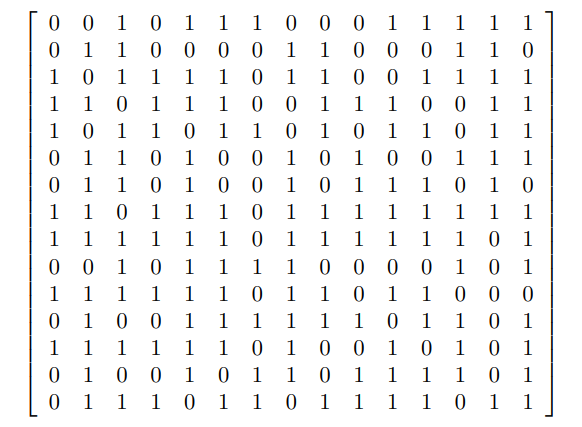
\includegraphics[scale=0.47]{Imagenes/matriz1.png}
    \caption{Matriz llenada con el método \textbf{\texttt{\textbf{fill}}}}
    \label{fill}
\end{figure}


\subsection{\textbf{Identificación de clusters percolantes}}

Una vez se tiene la matriz sobre la que se va a trabajar, para determinar si el sistema percola o no, se desarrollaron 3 funciones principales, sin embargo, el corazón del método se encuentra en la función llamada \texttt{\textbf{hood}}, esta función está pensada para que, dada una casilla abierta en la posición $(i,j)$ de una matriz $I$, y una matriz nula $F$, establece un valor objetivo (\texttt{\textbf{target}}), y un valor nuevo (\texttt{\textbf{new}}) que son pasados como parámetros de la función, entonces, si la posición $(i,j)$ contiene el valor objetivo, entonces el método buscará los vecinos de $(i,j)$ que también contengan el valor objetivo, es decir, identificará un cluster (percolante o no) formado por el valor objetivo, y en la matriz $F$ se copiará este cluster con el detalle de que este estará compuesto por el valor de \texttt{\textbf{new}}, este parámetro será de utilidad a la hora de encontrar el cluster percolante más grande.
\vspace{0.2 cm}

Con esta rutina principal es sencillo identificar los clusters percolantes, para esto se crearon las funciones \texttt{\textbf{path}} y \texttt{\textbf{cluster matrix}}, dado que es necesario identificar los clusters percolantes, es suficiente con usar el método \texttt{\textbf{hood}} en la primera y última fila, y en la primera y última columna de la matriz de estudio, garantizando que los lugares llenos de la mueva matriz $F$ pertenecerán únicamente a clusters percolantes, esto es lo que hacen los métodos \texttt{\textbf{path}} y \texttt{\textbf{cluster matrix}}, a la matriz resultante se le llamó \textit{matriz de percolación}.
\vspace{0.2 cm}

En la figura 2 se muestra un ejemplo del funcionamiento de las rutinas tomando la matriz de la figura 1.


\begin{figure}[H]
    \centering
    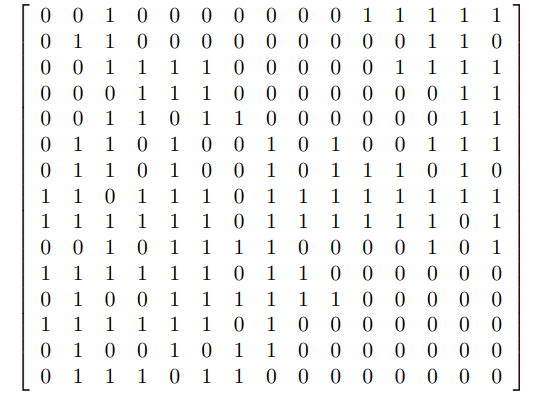
\includegraphics[scale=0.5]{Imagenes/matriz2.png}
    \caption{Matriz de percolación obtenida mediante los métodos \textbf{\texttt{path}} y \texttt{\textbf{cluster matrix}}. Cada casilla llena pertenece al cluster percolante}
    \label{hood1}
\end{figure}

Finalmente, una vez obtenida la matriz de percolación, se creó el método \texttt{\textbf{percolation}} de tipo \texttt{\textbf{bool}}, que recibe la matriz de percolación y escanea su primera fila y su primera columna en busca de un elemento diferente de cero, si al menos uno de estos elementos lo es, quiere decir que pertenece a un cluster percolante y por ende el sistema percola.




\subsection{\textbf{Determinación del cluster percolante más grande}}

Un hecho bastante aprovechable para obtener el tamaño del cluster percolante más grande, es que para que exista más de un cluster percolante, estos deben ser o solamente verticales, o solamente horizontales, si el sistema percola en las dos dimensiones, automáticamente todos los elementos abiertos en la matriz de percolación pertenecen al mismo cluster, por ende el tamaño del cluster más grande en esta situación será el tamaño de este único cluster.
\vspace{0.2 cm}

Con el fin de discernir las situaciones en las que se tiene percolación puramente horizontal o puramente verticial se creó la función \texttt{\textbf{sep}} cuya entrada será la matriz de estudio, y mediante el método \texttt{\textbf{path}} se devolverá una vector bidimiensional cuyos elementos pueden tomar el valor de 0 o 1, la primera componente será 1 si el sistema percola horizontalmente, y 0 si no, para la segunda componente se usa la misma regla con la diferencia de que esta representa la percolación horizontal.
\vspace{0.2 cm}

La estrategia general para encontrar el tamaño del cluster percolante más grande, fue asignarle un número entero positivo cada cluster percolante independiente, es decir, la indexación de los clusters percolantes. Para esto se desarrolló la función \texttt{\textbf{index matrix}}, la cual toma la matriz de percolación y, a cada cluster percolante y, haciendo uso de la función \texttt{\textbf{sep}} y la función \texttt{\textbf{hood}} con su funcionalidad de crear clusters cuyo número representante sea distinto, y devuelve una matriz en la que cada cluster percolante independiente tiene su propio número, a esta matriz de retorno se le llamó \textit{matriz indexada}. En las figuras 3 y 4 se ilustra un ejemplo de este método.
 \begin{figure}[H]
    \centering
    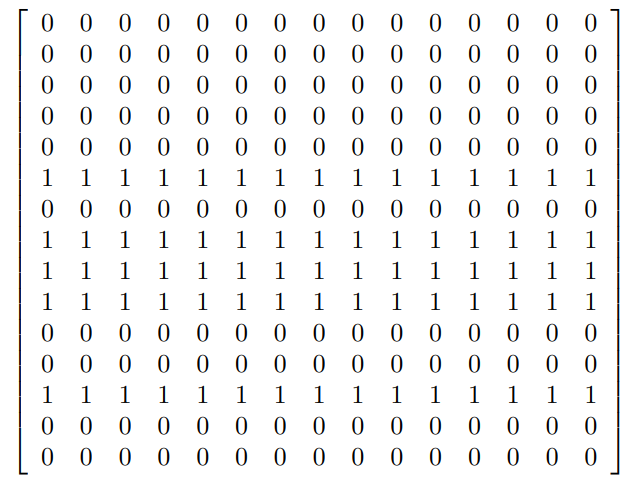
\includegraphics[scale=0.4]{Imagenes/matriz3.png}
    \caption{Matriz de percolación con clusters percolantes puramente horizontales.}
    \label{matrix}
\end{figure}


\begin{figure}[H]
    \centering
    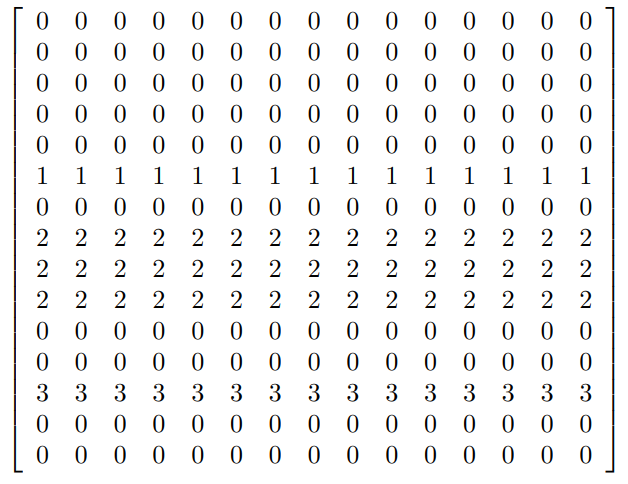
\includegraphics[scale=0.41]{Imagenes/matriz4.png}
    \caption{Matriz indexada.}
    \label{index}
\end{figure}

Una vez obtenida la matriz indexada, esta es ingresada a nuestra última función, llamada \texttt{\textbf{cluster size}}, que, toma la matriz indexada y mediante la librería \textbf{\texttt{vector}} es transformada en un arreglo unidimensional, y claramente, debido a que los clusters percolantes están indexados, el tamaño del cluster percolante más grande será el número de veces que aparezca el número de más repetido del arreglo unidimensional, este valor se determinó haciendo uso de los métodos \texttt{\textbf{max element}} y \texttt{\textbf{distance}}
de la librería \texttt{\textbf{algorithm}}.

\begin{verbatim}

\end{verbatim}





\section{\textbf{Identificación y solución de problemas}}
 \label{sec:problems}
 Al realizar un proyecto de computo es usual enfrentarse a diferentes dificultades, las cuales se sanearan de diferentes formas. La primera dificultad encontrada fue vista por un \textit{sanitizer adress}, se identificó que la función recursiva \texttt{\textbf{hood}} era llamada una cantidad de veces tan grande que consumía la memoria del \textit{stack}, por lo que al ejecutar el programa para tamaños mayores a $L=512$ y probabilidades mayores a $p=0.55$ se obtenía el \textit{sanitizer} anteriormente mencionado. \\
 Para solucionar este problema, se recurrió a buscar una forma de liberar memoria, para ello se forzó a una de las matrices intermediarias en el proceso de identificación de clusters a que al finalizar su uso se realizara un \textit{resize} a una matriz de tamaño nulo; lo cual incremento el rango en que se ejecutaba correctamente hasta valores de $1024$, con probabilidades de hasta $0.64$, un incremento notable que podría ser mejorado.\\
 Otro de las dificultades encontradas, no corresponde al algoritmo directamente, está relacionada al trabajo del proyecto a partir del uso de múltiples carpetas y dependencias; es decir, referido a compilación de múltiples archivos ubicados en diferentes carpetas, todas estás dificultades fueron solventadas a partir de un proceso de aprendizaje autónomo en el manejo de makefiles, bash y las múltiples opciones que el compilador ofrece.

\section{\textbf{Resultados y análisis}}
Para determinar la probabilidad $P(p,L)$ de que exista un cluster percolante y el tamaño promedio del cluster percolante más grande $s(p,L)$ se realizaron diferentes simulaciones descritas a continuación. \\
A partir de los algoritmos usados en la sección 2, la toma de datos en un conjunto de $L=\{32, 64, 128, 256, 512\}$ se hizo tomando 30 valores diferentes de $p$ entre $0$ y $1$, de los cuales 11 están en el rango $0.55$ a $0.65$. Para cada valor de $L$ y $p$ la simulación se hizo 10 veces y por cada vez se vario la semilla aleatoria de forma que cada vez se obtenían resultados distintos para el mismo valor de $L$ y $p$. Los datos obtenidos para cada valor de $p$, $L$ y $seed$ fueron: la existencia de cluster percolante, el tamaño del cluster percolante más grande y el tiempo de computo.

\subsection{\textbf{Probabilidad de que exista un cluster percolante}}
Con los datos obtenidos se calcula cuantas veces en promedio aparecía un cluster percolante, por ejemplo, para $L=32$ y $p=0.5$ se corrió la simulación 10 veces variando la semilla aleatoria, y se obtuvo que solo en 1 de los casos hubo cluster percolante, por lo que el promedio es $P(0.5,32)=1/10=0.1$ como se ve en la gráfica de la figura 5, también se calcularon las desviaciones estándar para cada promedio obtenido.
\begin{figure}[H]
    \centering
    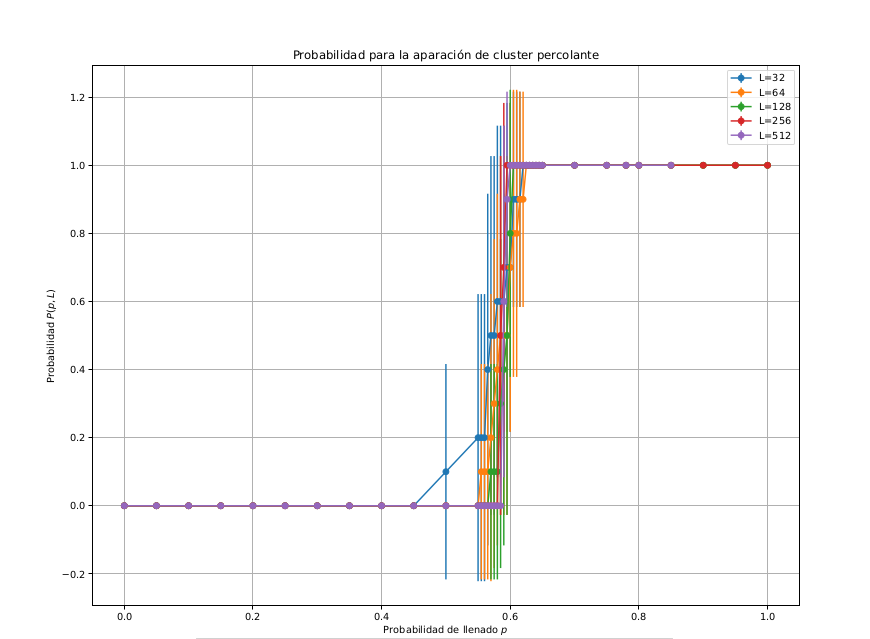
\includegraphics[scale=0.35]{Imagenes/Probabilidad.png}
    \caption{Probabilidad de la aparición de cluster percolante donde para cada valor de $L$ se varió la probabilidad de llenado $p$ para obtener valores de probabilidad que dependen de $p$ y $L$}
    \label{Promedio}
\end{figure}

Se puede observar que para valores superiores a $p=0.6$ se puede garantizar la existencia de cluster percolante sin importar su tamaño $L$ debido a que en promedio la probabilidad es igual a 1 y su desviación estándar es cero, es decir que todos los 10 datos obtenidos para cada variación de $p$ y $L$ con $p\geq0.6$ hay un cluster percolante. De forma similar para probabilidades menores $0.5$ se puede garantizar la no existencia de cluster percolante ya que como vemos el promedio es igual a 0 y su desviación estándar es nula.\\
Por último, se observa que el promedio es distinto de cero a partir de cierto valor dependiendo del tamaño de la matriz, así se tiene que entre más grande es $L$ esto sucedo cuando la probabilidad de llenado se acerca a $p=0.6$, por ejemplo para $L=32$ $P(0.5,32)=1$ por primera vez pero para $L=512$ el promedio se hace distinto de cero para $p=0.59$ muy cercano a $0.6$.

\subsection{\textbf{Tamaño del cluster percolante más grande}}
Con los datos obtenidos también se pudo calcular el tamaño promedio del cluster percolante más grande normalizado al tamaño total de la matriz $L\times L$ además de sus correspondientes desviaciones estándar (también normalizadas) como se muestra en la gráfica de la figura 6.

\begin{figure}[H]
    \includegraphics[scale=0.3]{Imagenes/TamañoDelCluster.png}
    \caption{Tamaño promedio del cluster percolante más grande donde se varió $p$ para diferentes valores de $L$ obteniendo valores para el tamaño del cluster percolante más grande, estos datos se normalizaron al tamaño de la matriz}
    \label{Tamaño}
\end{figure}

Se puede observar que el tamaño promedio para cada valor de $L$ aumenta conforme aumenta la probabilidad de llenado y vemos que tiende a ser igual a $L\times L$.

\subsection{\textbf{Tiempo de computo}}

Dentro del paradigma de la computación interesa saber como escala el tiempo de computo respecto al tamaño del sistema. Sin embargo, hay dos factores a considerar; el primero de ellos es el efecto del valor de la probabilidad $p$, debido a la influencia de este valor en la existencia o no de un cluster percolante y el uso de algoritmos recurrentes para hallarlos, se espera que un mayor valor de $p$ implique que la función \textbf{\texttt{hood}} tenga que ser llamada una mayor cantidad de veces, conllevando un mayor tiempo de computo; el segundo efecto es el uso de optimizaciones, en este caso proveídas por banderas del compilador, para este caso se evaluó el efecto sin optimizaciones \texttt{-O0} y con dos niveles diferentes de optimización (\texttt{-O1} y \texttt{-O3}). \\
\vspace{0.2 cm}

En las figuras 7, 8 y 9 se observa el tiempo de computo en función del tamaño del sistema para tres diferentes valores de probabilidad fija y los diferentes niveles de optimización mencionados.\\
Notese que el rango de la fig. 9 abarca hasta $M=250$.
\begin{figure}
    \centering
    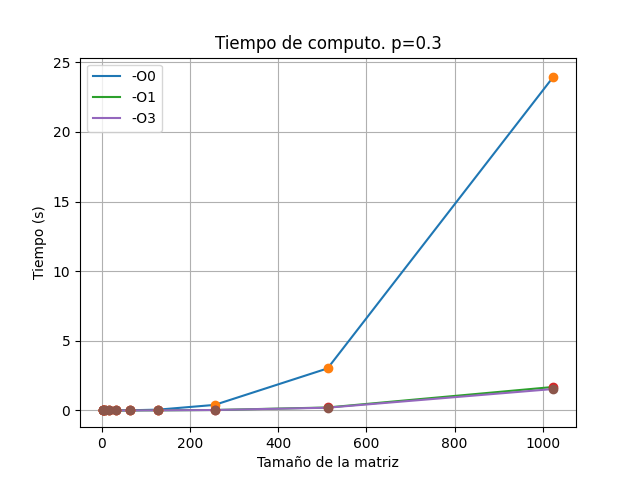
\includegraphics[width=1\linewidth]{Imagenes/Computing_time_p03.png}
    \caption{Tiempo de computo para $p=0.3$}
    \label{fig:Comptime03}

    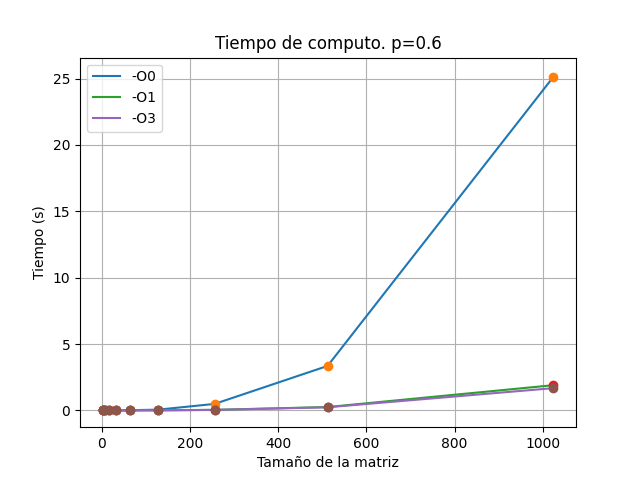
\includegraphics[width=1\linewidth]{Imagenes/Computing_time_p06.png}
    \caption{Tiempo de computo para $p=0.6$}
    \label{fig:Comptime06}

    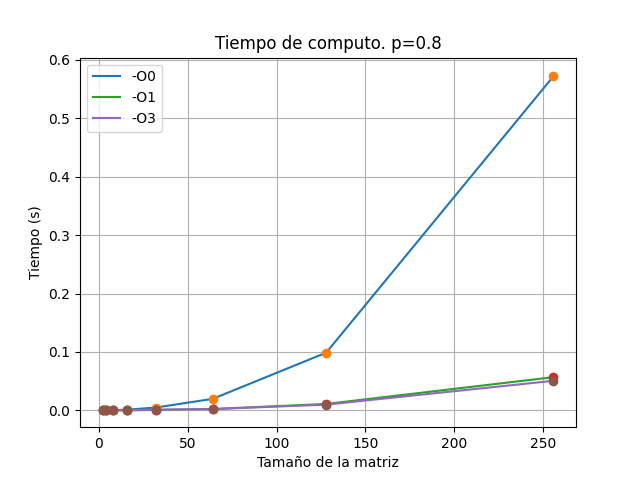
\includegraphics[width=1\linewidth]{Imagenes/Computing_time_p08.png}
    \caption{Tiempo de computo para $p=0.8$}
    \label{fig:Comptime08}
\end{figure}

\vspace{0.2cm}
De las figuras 7, 8 y 9 se determina que aunque el valor de la probabilidad tiene efectos en el tiempo de computo para cada valor de M, no tiene un efecto en la tendencia de la curva. Es posible ver que existe una gran diferencia entre \texttt{-O0} y \texttt{-O1}, es decir el compilador realiza un gran proceso de optimización disminuyendo el tiempo de computo en un $90\%$; no obstante, este es el único cambio significativo, ya que entre diferentes niveles de optimización el cambio está entre el $1\%$ y el $4\%$.\\
Para analizar el tiempo de computo también se hizo uso de herramientas de análisis de rendimiento, \textit{gprof}; en el archivo \texttt{profiling-report.txt} se puede ver el perfil de rendimiento del código para una ejecución con $L=128$ y un valor cercano a la probabilidad critica $p=0.60$, con el cual existía un cluster percolante en el sistema. Del reporte se pueden extraer varios detalles; el primero de ellos es el porcentaje de tiempo que gastan las funciones, se identifica cual es la función que consume casi la totalidad (valor cercano al 100\%), siendo \texttt{\textbf{cluster size}}, es decir la encargada de determinar el tamaño del cluster percolante más grande; también se identifico que la función recursiva \texttt{\textbf{hood}} fue llamada 94314 veces, un valor alto, el cual en este caso no genera problemas, pero debido al tamaño del stack, podrían generarse para sistemas más grandes, como se mencionó en la sección 3.

\section{\textbf{Conclusiones}}
La probabilidad con la cual se puede garantizar la existencia de un cluster percolante torna alrededor a $p=0.6$, tal y como se esperaba; la probabilidad de que exista un cluster percolante $P(p,L)$ depende del valor de $p$ y $L$ en el régimen de $p\in (0.50,0.60)$, ya que para valores menores al rango la probabilidad será nula, y para valores mayores será $1$. \\
El tamaño del cluster percolante mas grande también aumenta conforme aumenta la probabilidad de llenado $p$ tal y como se esperaba, como se ve en la gráfica de la figura 6 los tamaños del cluster percolante tienden a un valor máximo que corresponde al tamaño de la matriz, es decir $L\times L$, lo cuál corresponde a lo obtenido cuando la probabilidad de llenado $p$ es igual a $1$.

Se encuentra que la probabilidad de llenado afecta al tiempo de computo de tal forma que la tendencia no depende de ella; asimismo, se comprobó que el efecto de la optimización no depende de esta probabilidad y es apreciable cuando se cambia de \texttt{-O0} a \texttt{-O1}, pero el efecto no es visible entre los diferentes niveles de optimización. Por último se encontró que la función que es llamada en menor cantidad de veces y sobre la que se habría de trabajar es la función recursiva \texttt{hood}, es decir la  encargada de recorrer la matriz en busca de vértices llenos.

\printbibliography

\section{Referencias}
\begin{itemize}
    \item[[1]] Real Academia Española. \textit{Definición de percolar.} 2021. \texttt{URL}:https://dle.rae.es/percolar
    \item[[2]] Harry Kesten. <<What is... percolation?>> En: \textit{Notices of AMS} (2006). \texttt{URL}:https://www.ams.org/notices/200605/what-is-kesten.pdf
    \item[[3]] Eric Weisstein. <<Percolation site>>. En: \textit{Wolfram Matheworld} (2022). \texttt{URL}: https://mathworld.wolfram.com/SitePercolation.html
    \item[[4]] \textit{cpp reference / random.} \texttt{URL:}  https://en.cppreference.com/w/cpp/numeric/random
    \item[[5]] \textit{cpp reference / algoritm}. \texttt{URL:} https://en.cppreference.com/w/cpp/algorithm
    \item[[6]] \textit{cpp reference /vector.} \texttt{URL:}  https://en.cppreference.com/w/cpp/container/vector
    \item[[7]] \textit{Eigen} \texttt{URL:} https://eigen.tuxfamily.org/dox/
\end{itemize}
%Me voy,

\end{document}
